\chapter{Background}

This chapter will provide a general scientific context for this dissertation. First, a general outline of energetic ion-solid interaction is given. Next, the effects of the interaction between the ion and the electrons in the solid are discussed separately from the collisions of the ion with nuclei in the solid. With this background, the possibilities of simulating the ion-solid interaction are discussed with an emphasis on effects and literature relevant to the experiments in this thesis. 

\section{Ion-solid interaction}
\label{sec:ionsolid}

\subsubsection{Energy loss}

An energetic ion impinging on a solid will lose its kinetic energy $E$ to the solid over the distance traveled $x$ in a variety of processes. The stopping power $S$ is well described for a large energy range by the Bethe (sometimes ``Bethe-Bloch'') formula derived using the Born approximation perturbation theory on the impact between the `fast' ion and the `slow' electrons in the solid: 

\begin{equation}
S = \frac{dE}{dx} = - A \cdot \frac{\rho\,Z_2\cdot Z_1^2}{\beta^2} \cdot \left[ln\Big(\frac{B\cdot\beta^2}{Z_2\cdot(1-\beta^2)}\Big)-\beta^2\right] ,
\end{equation}


with $A$ and $B$ positive combinations of constants, $\rho$ the density and $Z_2$ the atomic number of the target, $Z_1$ and $\beta = v/c$ the atomic number and relativistic velocity of the ion. Corrections to this formula are especially necessary for low ion energies, but in detail they are dependent on the target composition, the ion energy and ion mass in a non-trivial way. Figure \ref{stopping} and the following discussion illustrates stopping regimes and why corrections are required to the Bethe formula. It is adapted from \cite{sigmund_stopping_2004}.

\begin{figure}
	\centering
		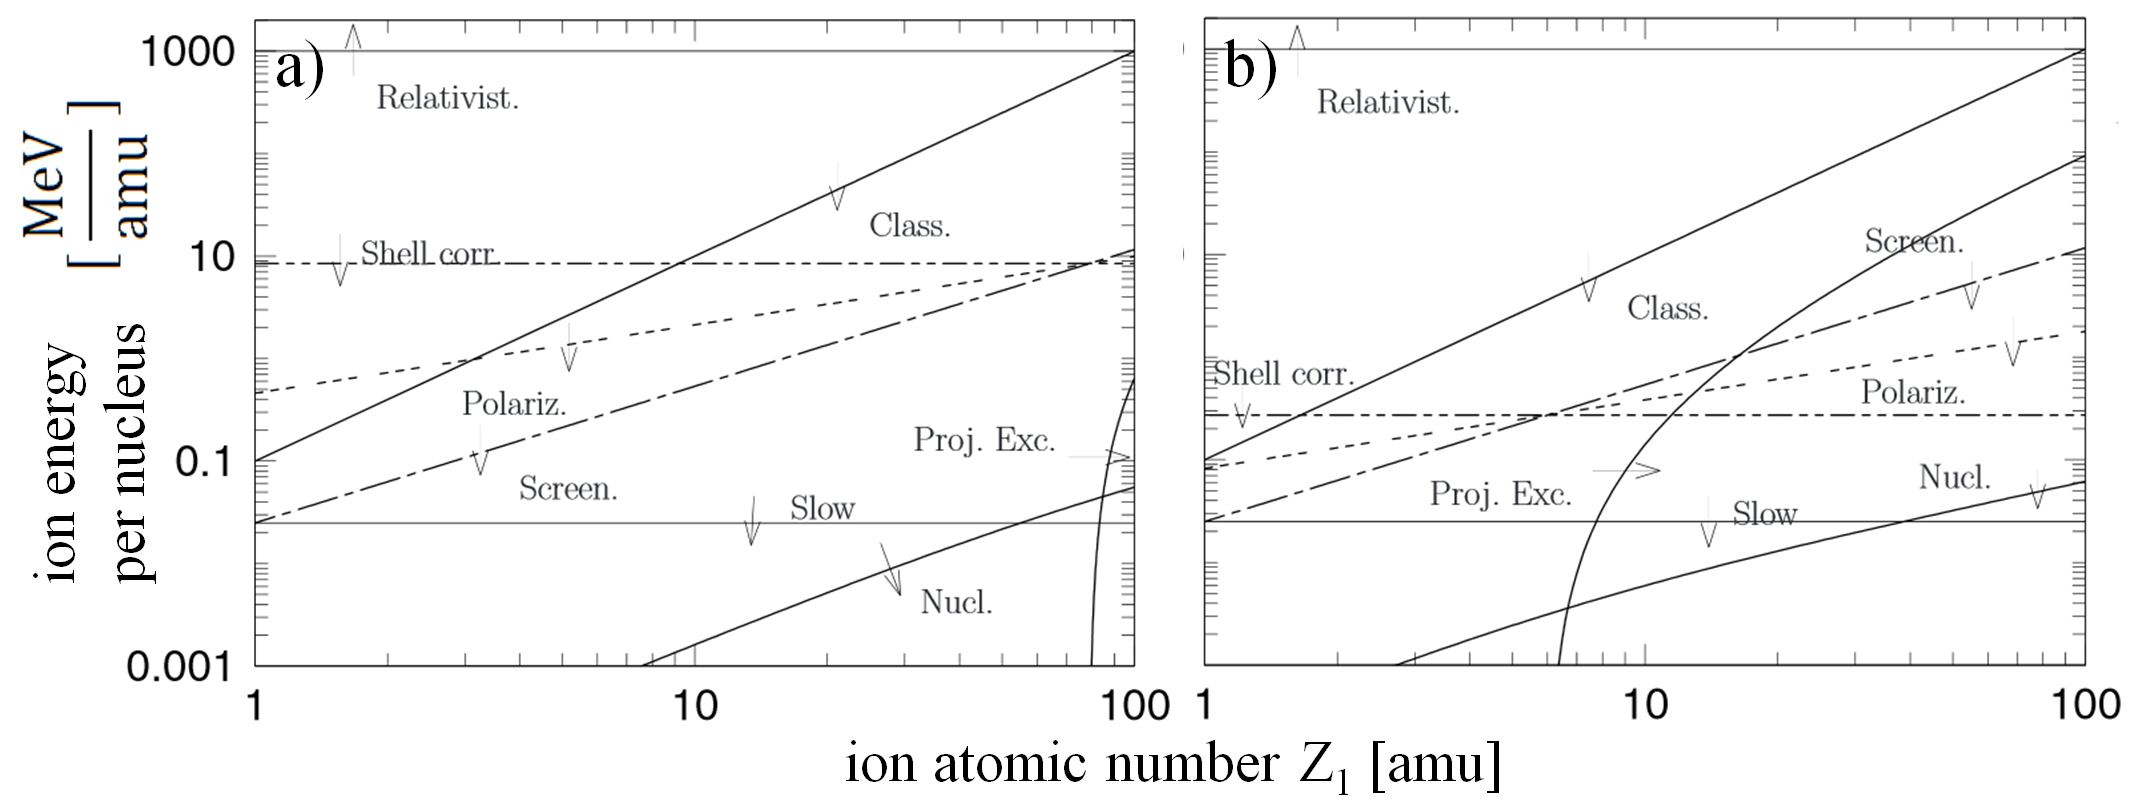
\includegraphics[width=.95\textwidth]{images/StoppinginAuandC.png}
	\caption{Illustration of the dominant effects on the stopping power for an ion of mass $Z_1$ and energy $E$ in $Au$ a) and $C$ b). Adapted from \cite{sigmund_stopping_2004}.} 
	\label{stopping}
5\end{figure} 

At high ion energies ($ > 1\,GeV/amu$, labeled ``Relativist.'') highly relativistic effects have to be taken into account. At these energies we have, for example, Cherenkov radiation. 

%Typically, nuclear reactions and resonances also occur at high ion energies. However, as nuclear reactions may change the ion species, their cross sections are usually treated separately from the stopping power.

The horizontal line labeled ``Shell corr.'' marks the Thomas-Fermi velocity ($Z_2^{2/3}v_0$) of the target electrons. The constant $v_0 = e^2/\hbar = 25\,keV/amu$ is the Bohr velocity. In the parameter-space below this line the ion is moving at speeds comparable to that of the electrons in the target. In the low energy area below the line labeled ``Slow'' ($25\,keV/amu$) the ion is traveling at speeds below the Bohr velocity of the target electrons. Here the ion velocity is only comparable to that of the valence electrons in the solid. Both these points mean that the actual electron density distribution and chemical nature of the solid becomes relevant, which is of course not considered in the general Bethe formula. This makes a general and accurate theoretical prediction of the stopping power impossible for low ion energies. Specific ion-target combinations require specific investigations.

Above the line showing the Thomas-Fermi velocity of the ion ($v = Z_1^{2/3}v_0$, ``Screen.'') the ion can be assumed to be stripped of all its electrons. Below, a screening function must consider the effective charge of the ion. Below the curve labeled ``Proj. Ext.'' the ion (projectile) carries a comparable number of electrons to the target making excitation processes in the electronic configuration of the ion significant.

For ion velocities $v < (Z_1Z_2)^{1/3}v_0$ (labeled ``Polariz.'') a higher order ($Z_1^3$) correction term to the Bethe formula becomes relevant due to the Barkas-Andersen effect. Below the line marked ``Class.'' ($Z_1^2\cdot 100\,keV/amu$) classical Bohr orbits can be used for electrons around the ion, this is a \emph{sufficient} criterion for the derivation of the Bethe formula not a \emph{necessary} one.

Finally, not be confused with the nuclear reactions already mentioned, in the region marked ``Nucl.'', at low ion energies and for large ions, the interaction with the electronic system becomes weak. Here the contribution of the coulomb interaction between ion and individual target atoms as a whole become the main contribution to slowing the ion. This is called nuclear stopping in contrast to the electronic stopping discussed so far, as kinetic energy is transferred to the target nuclei, not just the electrons. The effects that the ion irradiation has on the solid will be discussed next by looking at the electronic and nuclear energy loss separately. 

\subsubsection{Discussion of electronic energy loss}

 %For biological material

Electronic stopping $S_e$ is the sum of the interactions between the ion and the electrons in the irradiated solid. In the simplest case a target atom is ionized, followed by a host of effects such as characteristic X-ray emission and Auger electron emission associated with the relaxation of this excited state. Analogously, excitation in a semiconductor is associated with band to band, exciton etc. recombination. The luminescent and fluorescent relaxation mechanisms are, however, generally not very efficient. Most of the energy deposited in the electronic system will be turned into kinetic energy of electrons and subsequently converted to heat. This happens very locally on the $nm$ scale of the electrons mean free path and thus also very quickly, within the order of $ps$. 

% Detection of these emissions can be used for ion beam analysis (IBA) of the solid irradiated. A confident and comprehensive review of the possibilities of IBA can be found in reference \cite{jeynes_total_2012}.

The effects of such local heating on a solid are diverse. Defects and amorphous regions may either appear or disappear, depending on the material and its history. For large ion masses and energies (swift, heavy ions), the deposited energy density becomes large enough to form an ``ion track'' around the path of the ion. Ion tracks are a whole field of research outlined well by references \cite{toulemonde_transient_1992,miotello_revisiting_1997,wesch_effect_2004}. Very large electronic losses have to be treated carefully as a large percentage of the electrons within the track are energized and some electrons also gain a significant amount of kinetic energy. 

The energies used in this dissertation are in the order of $\approx 100\,keV$ with elements of mass $\approx 100\,amu$. The energy regime investigated in this dissertation is thus right at the bottom of the area plotted in figure \ref{stopping}. Electronic stopping is not dominant, so that it is sufficient to treat the electronic energy loss as a local heat source.

\subsubsection{Discussion of nuclear energy loss}

The seemingly more straightforward process in the energetic ion-solid interaction is an elastic collision between the impinging ion and a target atom. Its first observation was in the famous Rutherford (Geiger–Marsden) experiment \cite{rutherford_scattering_1911} which was groundbreaking to understanding the structure of matter. Nuclear energy loss is caused by the kinetic energy which is transferred form the energetic ion onto an atom in the target. An impinging ion can transfer considerable energy to an atom, which in turn will collide with other lattice atoms, leading to the formation of a collision cascade. This displacement of atoms from their lattice position is the main contribution to irradiation damage and sputtering of the target. 

The amorphization of crystalline semiconductors has been investigated extensively with a good review found in reference \cite{wesch_damage_2012}. The damage production depends a lot on the irradiated semi-conductor and on the density of the collision cascade caused by the irradiating ion. In general the defects produced by nuclear energy loss are Frenkel pairs. On further irradiation, interstitials and/or vacancies can agglomerate to form extended defect clusters which initiate amorphization. The fluence at which the material is amorphized is highly temperature dependent as Frenkel pairs can anneal at high implantation temperatures. This can lead to an arbitrarily high amorphization fluence, if the annealing of defects is faster than their creation. A typical `radiation hard' material is $ZnO$ which is not amorphous even after $10^{17}\,cm^{-2}$ of $\,200\,keV\,Ar^+$ irradiation at $15\,K$ \cite{wesch_damage_2012}. An arbitrarily large amorphization threshold can also be obtained for $Si$ irradiated with $300\,keV\,Ar^+$ at $300^\circ\,C\,(\approx 600\,K)$ \cite{pelaz_ion-beam-induced_2004}.

In addition to the activation of defect recombination by increasing the `global' temperature, an increased local temperature by the energy deposited by the ion will also lead to `dynamic annealing'. The reduction of structure sizes leads to larger dynamic annealing as there is less material into which the energy deposited by the ion can dissipate, leading to higher local temperatures. This was shown in the $Mn$ irradiation of $GaAs$ nanowires \cite{borschel_ion-solid_2012,johannes_ion_2015} and could be used to improve the magnetic properties of the $GaAs:Mn$ nanowires \cite{borschel_new_2011,paschoal_hopping_2012,kumar_magnetic_2013,paschoal_magnetoresistance_2014}. 

%In a recent study \cite{thome_recovery_2015} the dynamic annealing was enhanced by the simultaneous irradiation with $36\,MeV\,W$ a swift, heavy ion leading to predominantly electronic energy loss and $900\,keV\,I$ leading to large nuclear losses. Simultaneous irradiation lead to much less damage in the irradiated $SiC$ than subsequent irradiation. 

\subsubsection{The binary collision approximation}

A typical assumption in the theoretical treatment of nuclear energy loss is the binary collision approximation (BCA) for the ion and the target atoms. Under this assumption nuclear stopping is treated as a series of collisions between single particles. With the additional assumptions of 1) a spherically symmetric interaction potential and 2) the neglect of possible electronic effects (chemical binding) between the collision partners, the angular-momentum is conserved in the collision and the classical scattering-integrals can be solved. 

The resulting trajectories of a $Si-Si$ collision at $10\,eV$ is plotted in figure \ref{SiSi}. The large difference between the Moliére screened Coulomb potential and the $Si-Si$ potential derived by Dirac-Fock-Slater code is clearly visible. The former is a purely repulsive Coulomb interaction, while the latter includes an attractive interaction for large interatomic distances similar to the well known Lennard-Jones potential \cite{eckstein_computer_1991}. For high energy collisions a ``universal'' Ziegler-Biersack-Littmark (ZBL) potential based on a screened Coulomb interaction is quite successful \cite{ziegler_stopping_1985}, however for low energy collisions a generalized formula cannot be accurate and specific potentials have to be developed for each combination of collision partners \cite{dedkov_interatomic_1995,nordlund_repulsive_1997,albe_modeling_2002,nordlund_interatomic_2008}.

\begin{figure}
	\centering
		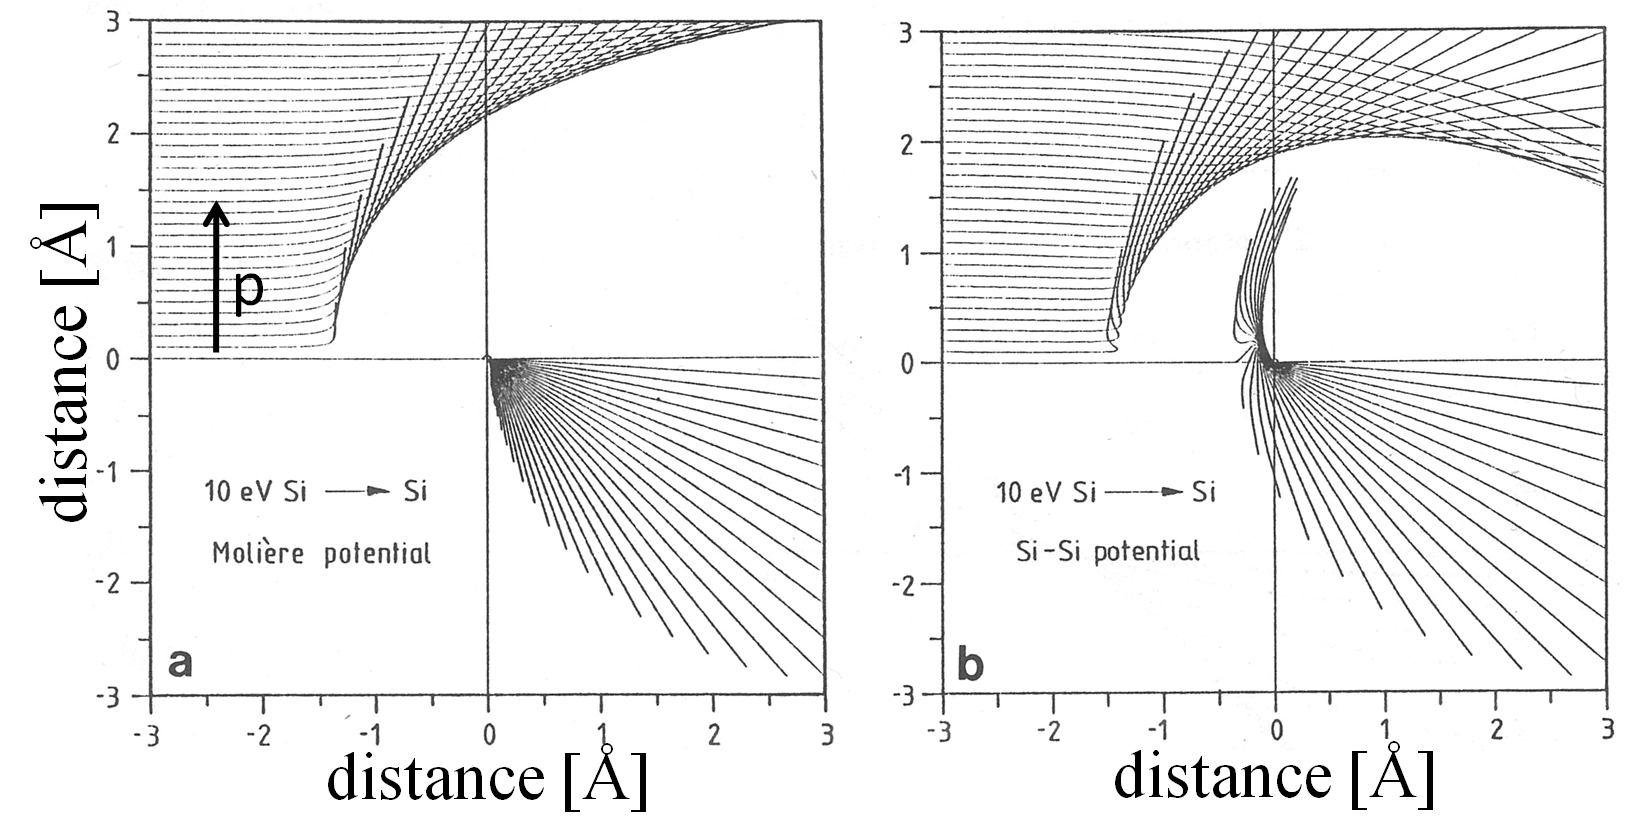
\includegraphics[width=.6\textwidth]{images/SiSicollision.jpg}
	\caption{Trajectories of a $10\,eV$ $Si-Si$ collision for a) Moliére and b) $Si-Si$ potential. The trajectories end after the same elapsed time for each impact parameter p. Adapted from \cite{eckstein_computer_1991}.}
	\label{SiSi}
\end{figure} 

In addition to this problem of finding the correct interaction potential for a collision, depending on the ion and the atomic structure of the irradiated material, the collision parameters relevant to low energy collisions are within the order of the inter-atomic distance of a few \AA, see figure \ref{SiSi}. The assumption that this is still a binary collisions can no longer be valid. In conclusion, it has to be noted that similar to the electronic stopping case, the assumptions for a generalized treatment of nuclear stopping are well fulfilled for large ion energies, but lose their validity at low energies $\ll\,1\,keV$.

\subsubsection{Sigmund theory of sputtering}

A prominent role in this dissertation will be played by a special effect of nuclear energy loss arising when the path of a recoiled atom intersects the targets surface: sputtering. The foundation of sputter theory was laid by Sigmund \cite{sigmund_theory_1969}. It is outlined in the following. The nuclear stopping of ions leads to the formation of highly branched collision cascades and most of recoiled atoms are found at the end of the many branches. Because of this, the majority of sputtered particles has a low energy and thus a low range in the material \cite{thompson_energy_1968}. They must thus originate from the surface of the target and the sputter yield, as the number of atoms sputtered per impinging ion, can be estimated by calculating the nuclear energy loss at the surface of the irradiated material and dividing it by a factor to account for the probability of an atom leaving the solid. 

The probability for the atom to leave the solid includes geometric considerations and the `surface binding energy' (SBE). A possible model for an atom leaving a solid is that of a potential plateau with the height of the enthalpy of sublimation which has to be overcome by the atom approaching the surface. This equates the energy required for sputtering an atom to the thermal energy required for sublimation. For metals this is a good assumption, as the metallic bond is undirected and mediated by the electron gas. However, the SBE model for sputtering neglects all effects related to the directionality of the local binding forces experienced by the atom to be sputtered and the modification of the surface by repeated removal of atoms, which will be relevant in compounds with covalent and ionic bonds.  

A reasonable assumption for the mean nuclear energy deposition distribution is a Gaussian ellipsoid, with the center at the ion range and the longitudinal and lateral straggling naturally defining its extensions. This approach was used by Sigmund to arrive at a good explanation for the energy dependence of sputtering from flat surfaces. Starting a low energies, the sputter yield will initially increase with increasing energy, simply due to more energy being available. For further increasing energy, however, the ion range becomes larger, leading to a predominant deposition of the energy deeper inside the target, away from the surface. A maximum is thus found at energies where the ion range is in the order of the longitudinal straggling. The angle dependence of sputtering can also be explained by the increased deposition of energy near the surface for larger angles of incidence, as shown in figure \ref{anglesigmund}.

\begin{SCfigure}[50][th]
	\centering
		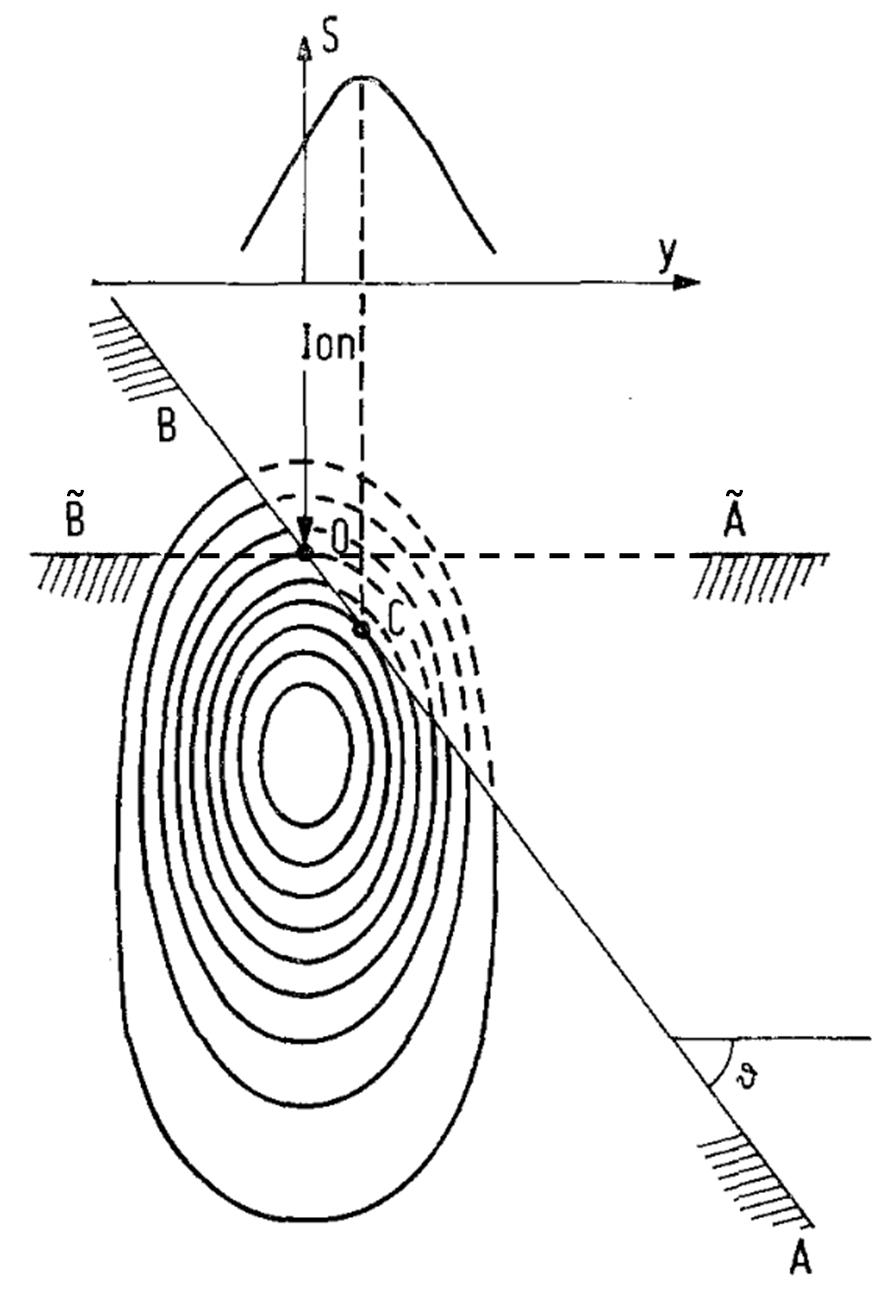
\includegraphics[width=.35\textwidth]{images/anglesigmund.jpg}
	\caption{Illustration of the Sigmund model of sputtering for irradiation of a bulk sample at an angle $\theta$. The ion enters the target at the point O and deposits the nuclear energy as indicated by the oval contours. The energy deposited along the inclined surface $BA$ is larger than that for the perpendicular surface $\widetilde{BA}$ leading to increased sputtering for irradiation at an angle. Also the deposited energy and thus sputtering is not largest exactly at the point of incidence O, but further down at the point C. This is illustrated by the projection of the sputter yield `S' onto the lateral dimension `y'. Adapted from \cite{sigmund_mechanism_1973}.}
	\label{anglesigmund}
\end{SCfigure} 

The Sigmund theory can also been applied to more complex surfaces. The Bradley-Harper theory of ripple formation on ion irradiated planes relies on the anisotropic sputtering predicted by the Sigmund model applied to a structured surface \cite{sigmund_mechanism_1973,bradley_theory_1988}. The increased sputtering at a point (C) downstream from the point where the ion enters the target (O) leads to an enhancement of surface roughness.

The Sigmund theory predicts a maximum in sputtering where the ion range is comparable to the nanostructure diameter. This can be understood by considering sputtering for a fixed ion energy and varying diameter, illustrated in figure \ref{radiussigmund}. At large diameters atoms can only be sputtered from the surface facing the ion beam. The sputter yield will still be larger than for a bulk sample as the local angle of irradiation is increased for non central impacts (A in figure \ref{radiussigmund}). For decreasing diameters the curvature of the wires increases, further increasing the intersection area between the estimated energy distribution and the nanowire (B in figure \ref{radiussigmund}). Once the diameter is in the order of the ion range, `forward' sputtering along the direction of the ions initial path will become possible (C in figure \ref{radiussigmund}). There is a maximum sputter yield for a radius comparable to the ion range, as the total surface area shrinks as $1/r^2$, reducing the sputter yield again for decreasing diameters. 

This model is obviously limited, as the nuclear energy distribution is assumed to remain constant even if the target surface intersects it (dashed lines in figure \ref{anglesigmund}). The maximum in the Gaussian ellipsoid approximation of the mean nuclear energy deposition is found where many of the branches of collision cascades overlap. A constant distribution wrongly includes those ion paths that would have left the nanostructure, as shown by the dashed ion trajectory in figure \ref{radiussigmund}. The more detailed description of the process thus required is outlined in the following section on the simulation of ion-solid interaction.

\begin{SCfigure}[50][t]
	\centering
		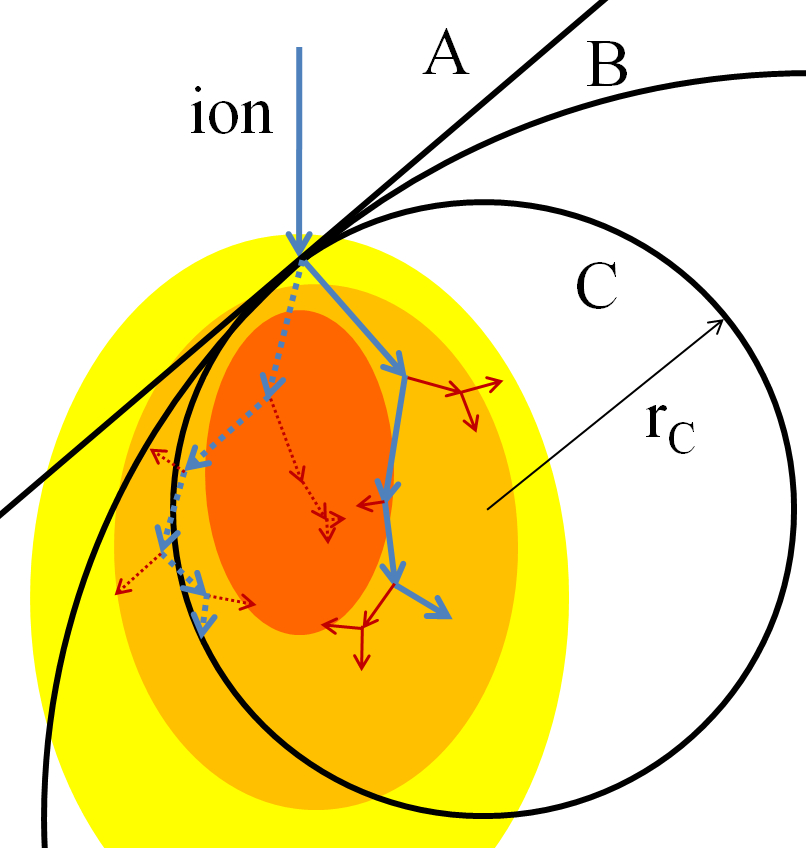
\includegraphics[width=.35\textwidth]{images/radiussigmund.jpg}
	\caption{Illustration of the Sigmund model of sputtering for irradiation of a curved surface. For an infinite curvature radius (straight line A) a non-central impact is the same as irradiation at an angle, as shown in figure \ref{anglesigmund}. For decreasing radii (B) the intersection between the colored energy distribution and the surface is increased. For small radii ($r_C$, C) forward sputtering appears. Two exemplary ion paths contributing to the colored average energy distribution are shown. The dashed path leaves and returns to the the smallest structure C.}
	\label{radiussigmund}
\end{SCfigure} 


\section{Simulation of ion-solid interaction}
\label{sec:simion}

In practice, the theory of ion-solid interaction is implemented in simulation tools which allow the experimenter to predict experimental outcomes. Most frequently the energy dependence of the ion range is obtained by simulations and used to decide which energy and fluence of irradiation is needed to create a desired doping concentration profile. On a more fundamental level, an experimentally observed behavior can be understood better by comparing it to various simulations to discern the dominating effects. The two main simulation approaches used for the ion-solid interaction are Monte-Carlo (MC) and molecular dynamic simulations (MD), both outlined in the following sections.


\subsubsection{Monte-Carlo simulations}

Monte-Carlo codes are simulation codes that use random numbers for simulations. After numerous simulations with different randomized outcomes, a statistical approximation of the likely outcome can be derived. With the BCA, the solid ion-interaction lends itself very well to MC simulation, as the evolution of a collision cascade can be simulated by following the paths of the ion and all recoils re-iteratively from one collision event to the next. The probability of a collision can be determined from the cross-sections determined by the interaction potential between the projectile and the atoms in the target. According to this probability, a randomized distance traveled in a straight line by the projectile is determined. The particle's kinetic energy is reduced by the electronic energy loss accordingly. This has the underlying assumption of a `random material' and crystal structure effects such as channeling are not reproduced by such a simulation. Two further random numbers are used to determine the impact parameter and azimuthal angle. The trajectories of the projectile and target atom in the plane of impact after the impact are determined by this impact parameter, the interaction potential and the particle energy, as shown in chapter \ref{sec:ionsolid}, figure \ref{SiSi}.

Examples of simulation codes implementing this approach in planar targets are TRIDYN \cite{moller_tridyn_1984}, SDTrimSP \cite{bizyukov_morphology_2008}, corteo \cite{schiettekatte_fast_2008}, COSIPO \cite{hautala_nuclear_1984} and, by far the most popular, SRIM \cite{ziegler_srim_2012}. In TRIDYN and SDTrimSP the target composition can be `dynamic', changing with the incorporation of ions and with selective sputtering of target atoms and the incorporated ions. It is clear from the discussion of chapter \ref{sec:ionsolid}, figure \ref{radiussigmund} that the irradiation of a nanostructure can not be approximated well with a planar simulation. Therefore, the recently developed TRI3DYN \cite{moller_tri3dyn_2014} and \emph{iradina} \cite{borschel_ion_2011} run a BCA MC simulation in a volume subdivided into rectangular voxels containing either vacuum or material to represent a three dimensional, structured target. TRI3DYN even includes dynamic composition and structural relaxation during the irradiation on a three dimensional simulation volume, but unfortunately it is not publicly available yet. Several \emph{iradina} simulation results will be discussed in this thesis, so the following points on the expected accuracy have to be made. 

The strong point of MC BCA simulations in general is that the direct simulation of the ion trajectories gives an accurate prediction of the final distribution of the ions in the target. This is a result of the sufficient accuracy of the previously discussed underlying theory of the energy losses for high energies. These predominantly determine the distance traveled by the ion in a collision cascade and also the distribution of nuclear and electronic energy loss. As the simulation directly follows the ions path, this accuracy can be expected to be upheld in the irradiation of nanowires. The concentration of incorporated ions is somewhat lower in nanowires than in bulk targets, as in a nanowire there are more possible paths that lead to the ions being scattered out of the nanowire, than there are in the irradiation of a bulk surface, see chapter \ref{sec:ionsolid}, figure \ref{radiussigmund} and reference \cite{borschel_ion-solid_2012}. 

Predicting the damage caused in the material by nuclear energy loss is a much more difficult prospect. The \emph{iradina} code checks at each collision whether the target atom acquires more energy than the ``displacement energy'' which is a material specific parameter. If an atom has less than the displacement energy after a collision, it is assumed to remain bound in its place and the energy is converted into lattice vibrations ($=$ heat). Atoms with more energy are displaced, creating a Frenkel pair which is counted as an interstitial at the location where the atom finally comes to rest and a vacancy at its point of origin. The displacement energy is experimentally accessible for crystalline materials by electron irradiation experiments in which the irradiating electron energy is in the order of $MeV$. From the electrons' impulse and mass the maximum transferred energy can be calculated. The defects produced as a function of electron energy can thus be used to determine a threshold energy for point defects, and this value is defined as the displacement energy. This not possible for amorphous materials, where point defects are ill-defined. Also, the number of Frenkel pairs this simulation creates is only an estimation at the \emph{creation rate} of the defects. The critical role that defect mobility, agglomeration and annealing plays in irradiation damage is totally neglected \cite{nordlund_correction_2014}.

Better results can be expected for the computation of sputtering, for which an excellent review is given in reference \cite{biersack_computer_1987}. The difficulty is that for low projectile energies the interaction with both the nuclear and the electronic system are not generalizable, as discussed in chapter \ref{sec:ionsolid}. This is a problem, as the dominating contribution to sputtering is made by low energy recoils \cite{thompson_energy_1968}. The various relevant interaction potentials however differ most at low energies. In addition, the SBE model used for Sigmund sputtering is just an approximation of the complexities arsing at real surfaces. For metals the situation is most favorable and in reference \cite{biersack_computer_1987} sputter yields of various metals are reproduced quantitatively. More recently, in reference \cite{hofsass_simulation_2014} by Hofsäss et al., good results on the sputtering of $Si$ and $Ge$ were obtained using the $Kr-C$ \cite{wilson_calculations_1977} potential which was found to be superior to the ZBL potential \cite{ziegler_stopping_1985}. Only the ZBL potential is implemented in \emph{iradina}, however, neither the $Kr-C$ nor the ZBL potential reproduce the angle dependent potential covalently bonded solids such as $Si$ \cite{stillinger_computer_1985,tersoff_new_1988}. Radially symmetric potentials are always only an approximation and which potential provides the better approximation in which scenario is not generally clear.

Hofsäss et al. also report a change in the dependence of sputtering on the angle of incidence for different interaction potentials. This might be worrisome even for the qualitative dependencies in the irradiation of nanostructures investigated in this thesis. However, the effect of different potentials on angle dependent sputtering is caused by the change in the critical angle for scattering at the surface of the impinging ion, not by a later change in the distribution of the nuclear energy deposition within the target. Since the critical gracing incidence angle is close to $0^\circ$ regardless of the interaction potential for the relatively high energies ($\approx\,100\,keV$) used in this dissertation \cite{yamamura_empirical_1984}, the accuracy of qualitative predictions will be unaffected. Finally, Hofsäss et al. also investigated the compounds $Ta_2O_5$ and $SiO_2$ finding that dynamic simulations are necessary, as preferential sputtering and composition changes play a significant role. This is not possible in \emph{iradina} and will be discussed where relevant.


Even though \emph{iradina} can implement an analytical description of a cylinder, most of the simulations in this work were nevertheless performed on the voxel based simulation volume, as this granted more freedom in the creation of the simulation volumes. A typical simulation volume is shown in figure \ref{voxel}. The number of target atoms leaving the simulation volume per impinging ion gives the sputter yield. To ensure \emph{iradina} accounts for the surface binding energy correctly, the outermost voxel of the simulation volume has to contain vacuum, so that a sputtered atom makes a material-to-vacuum transition inside the simulation volume. Where the axial distribution was not relevant, the voxel $z$-size was set to $10\,nm$ with periodic boundary conditions. The accuracy of the approximation of a curved surface in the $xy$ direction, such as the surface of the cylindrical nanowires, is obviously dependent on the voxel size. Since the surface of the approximation by rectangular voxels of a cylinder is strictly larger than the analytical surface, sputtering may be slightly increased. Also, the possible ions' impact angles are limited to the angle between the ion beam and the plane surfaces of the voxels facing the ion beam, so that the impinging angle is always larger in the voxelated surface than for the analytical surface. However, this will have no large effect, since, as before, the small critical angles for reflection of ions are restricted to the very outermost edges of the nanowire. Considering these effects, it was found that for voxel edges of $2\,nm$ and below only a negligible influence of the voxel size on the sputtering remained. 

\begin{SCfigure}[50][h]
	\centering
		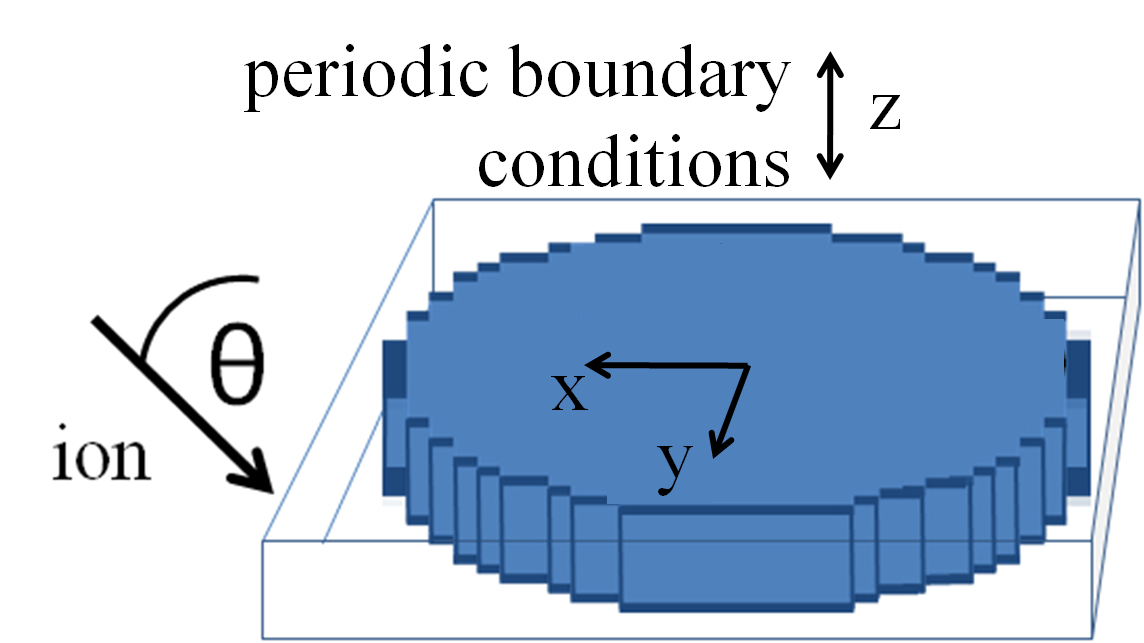
\includegraphics[width=.5\textwidth]{images/voxel.jpg}
	\caption{Typical implementation of a nanowire for an \emph{iradina} simulation. The ions enter the simulation volume at $x=0$; $y,z=random$ with an angle to the $z$-axis of $\theta = 45^\circ$. The $z$-direction is periodically continued. The $x$ and $y$ direction have $102$ voxels of $0.02-2\,nm$ edge-length so that nanowire with diameters of $2-200\,nm$ can be simulated.}
	\label{voxel}
\end{SCfigure} 

In summary, the prediction of sputtering as simulated by \emph{iradina} in this thesis is expected to be dependable with respect to the qualitative relationship between ion range and structure size, and sputtering. Quantitative sputter yields will, however, be inaccurate.


\subsubsection{Molecular dynamic simulations}

The MC BCA simulations outlined so far inherently neglect all effects occurring when more than two particles move at the same time. Molecular dynamic (MD) simulations, however, follow the path of every particle in the simulation volume individually, calculating the interaction potential between them at every time step \cite{alder_studies_1959}. Obviously this is much more computationally expensive than the BCA and simulation volumes and times are thus limited. Nevertheless the method can be applied to ion irradiation \cite{nordlund_molecular_1995} and increasing computer power has led to the simulation of ever higher particle energies, which require a larger simulation volume and time \cite{greaves_enhanced_2013,baumer_prediction_2014,anders_sputtering_2015}. The interactions between the target atoms in the MD simulations have to recreate the atomic structure, thermal vibrations etc., so that the low energy regime of the interaction potential is critical and has to be adapted to the specific problem \cite{dedkov_interatomic_1995,nordlund_repulsive_1997,albe_modeling_2002,nordlund_interatomic_2008}. Electronic energy loss can be included as a frictional force, however, treating this energy in a consistent manner is a problem, as the electronic system is typically not explicitly represented. Since MD simulations can reproduce the thermal evolution of a system, references to relevant MD simulation studies will be included in the discussion of results in this thesis.


\subsubsection{Relevant simulations in literature}

Two recent investigations on sputtering of spherical \cite{nietiadi_sputtering_2014} and cylindrical \cite{urbassek_sputter_2015} nanostructures have to be mentioned here as they overlap significantly with the studies made in this thesis. These publications have found the Sigmund model to be a decent first approximation for sputtering as it was discussed in chapter \ref{sec:ionsolid}. They go on to compare the sputter yield results from MC and MD simulations and discuss its diameter dependence. Unfortunately, the nanowire diameters investigated by MD are quite small owing to the computational costs. They find that for decreasing nanostructure diameters sputtering of clusters and thermal evaporation become increasingly important due to the lower number of atoms amongst which the ion deposited energy is distributed. This dissertation adds to results of these studies with simulations of diameter and energy dependent sputtering of nanowires in chapter \ref{sec:simsputering} and an experimental investigation of this dependency in the following chapter \ref{sec:sisputtering}.


\chapter{Experimental Methods}

\section{Nanowire synthesis}

Nanowire synthesis can be categorized according to two approaches: ``bottom-up'' and ``top-down''. The ``bottom-up'' approach relies on the self-organized arrangement of matter using an inherent anisotropy in the growth mechanism to create nanoscale structures. Depending on the material, crystal quality, morphology, infrastructural requirements, the quantity to be produced etc. there is a large variety of processes available for synthesis. The $ZnO$ \cite{borchers_catalyst_2006, stichtenoth_dimensionseffekte_2008, muller_structural_2009,ogrisek_kontrolliertes_2013}, $GaAs$ \cite{borgstrom_size-_2004, wacaser_preferential_2009} and $Si$ \cite{lugstein_pressure-induced_2008} nanowires investigated in this dissertation were grown using vapor transport, MOVPE and chemical vapor deposition respectively. 

A very common mechanism to create the anisotropy required to get the one dimensional growth of nanowires is the vapor-liquid-solid growth (VLS) first described by Wagner and Ellis \cite{wagner_vapor-liquid-solid_1964}. The variety of processes listed before are responsible to provide the `vapor' of material for this growth mechanism. With the vapor transport technique the source material eg. $ZnO$ is simply evaporated in a typically inert atmosphere and transported within a reactor to the substrate by diffusion or gas flow. Chemical vapor deposition uses reactive gases such as $SiH_4$ to provide the source material, in this case $Si$ in a temperature and pressure controlled reactor. Similarly in MOVPE a metal-organic gas is used as at least one of the sources, for example TMG (trimethylgallium) and $AsH_3$ to grow $GaAs$.

Although self-catalyzed growth has also been observed, the liquid part exploited in VLS is typically provided by a metal catalyst deposited on the growth substrate. The material in the vapor phase can accumulate in the catalyst droplet until the concentration is supersaturated. Preferential segregation of the excess material at the droplet-substrate interface leads to the growth of a nanowire. The size of the droplet can be used to control the diameter of the grown nanowire to some extent. The the growth of the ``bottom-up'' nanowires used in this thesis relies on the VLS mechanism. An epitaxial relation between the substrate and the nanowire material may be used to direct the growth. Typical nanowire diameters and lengths are $50 - 300\,nm$ and $> 5\,\mu m$ respectively.

Nanowires can also be synthesized ``top-down''. A ``top-down'' approach requires a predefined template which is used to control the desired morphology. The $Si$-nanowire arrays used to study sputtering and plastic deformation within this dissertation were etched by reactive ion etching (RIE) through a circular, e-beam lithographically defined $Ni$ hard-mask which set the nanowire diameter \cite{johannes_anomalous_2015}. Using the ``top-down'' etching process it is possible to prepare nanowires with diameters varying from $50\,nm$ to $2\,\mu m$ with a height of $\approx 3\mu m$ on a single substrate for simultaneous irradiation. The spacing between the nanowires was set to larger than their height, so that there is no shadowing of the ion beam between the nanowires.

Since the growth of nanowires was performed mainly by collaborators in Lund University ($GaAs$) and TU Vienna ($Si$) and is not part of the investigations reported here, the inclined reader is redirected to the cited references for further details respective growth parameters and their determination.

\section{Modification}


\subsubsection{ROMEO}


The ion irradiation for this dissertation was performed at the general purpose High Voltage Engineering implanter ``ROMEO'' at the IFK in Jena. It can provide an ion beam of virtually any element at energies ranging from $10-380\,keV$. The beam passes a $90^\circ$ selector magnet and can be sweeped with a frequency of $\approx 1\,kHz$ to homogeneously irradiate areas up to several tens of $cm^2$ with ion currents of up to $1\,mA$. For this work ion current densities were limited to $500\,nA/cm^2$, corresponding to $\approx 15\,min$ for the typical fluence of $10^{16}\,ions/cm^2$.

As a previous work has shown that nanowires can bend under ion irradiation \cite{borschel_permanent_2011, borschel_ion-solid_2012}, a rotatable and heatable, tilted stage (RHT) was custom built \cite{noack_sputter_2014}. With it, bending of the upstanding nanowires can be avoided as they are irradiated homogeneously from all sides at an angle of $45^\circ$. All the samples investigated in this thesis were rotated on the RHT and its preceding prototype sample stages during the irradiation. 

The sputtering and plastic deformation studies in chapters \ref{sec:sisputtering} and \ref{sec:quantifydeformation} were conducted with $Ar^+$ irradiation in $Si$ nanowires to avoid any chemical effects of the incorporated ions. To prevent defect induced density changes and the $Si$ nanowires from amorphizing, the irradiation temperature was $300^\circ$ for the sputtering study. At this temperature the amorphization threshold becomes arbitrarily high \cite{pelaz_ion-beam-induced_2004}. The other irradiations were performed at room-temperature. For the quantification of dopants $ZnO$-nanowires were irradiated with $Mn^+$. First $Mn$ has a similar mass to $Zn$ and both are medium-weight so that the linear cascade theory is applicable. Also, $ZnO:Mn$ is interesting as a possible material for diluted magnetic semiconductors (DMS) \cite{furdyna_diluted_1988,norberg_synthesis_2004}. Pragmatically, it is relatively easy to get a stable $Mn^+$ beam with ROMEO and with the quantification in mind, $Mn$ is much less likely to be in any components and give a background than $Fe, Co, Ni$ or $Cu$.

 
%RHT Bild?

\subsubsection{Focussed ion beam - FIB}

%hier ist noch blabla drin:
Some sample preparations required a FIB. They are highly specialized ion accelerators with the main objective of obtaining a small ion beam focus. Most of the systems use a $Ga^+$ beam and acceleration voltages up to $30\,keV$. The main use for FIBs is to sputter material extremely locally, making it a versatile tool for nano-machining. The FEI DualBeam Helios NanoLab 600i FIB system used for this dissertation is a scanning electron microscope (SEM) - FIB combination. The sample can thus be milled with the ion beam and investigated with the SEM re-iteratively. The system is also equipped with a $Pt$-metal-organic gas injection system. The $Pt$ containing organic molecule can be cracked locally on the sample by the secondary electrons created by either the electron or the ion beam. The FIB system can thus mill and deposit structures on a $nm$ scale. For the sample preparation in this thesis all $Pt$ deposition was done with the electron beam. Most of the $Pt$ is deposited near the impact point of the primary beam at the substrate. However, typically a rather large `halo' of minor $Pt$ deposition can extend for a couple of $\mu m$. 

\section{Characterization}

\subsubsection{Scanning Electron Microscope - SEM}

The morphological changes in the nanowires were characterized by high resolution SEM in the FEI DualBeam Helios NanoLab 600i FIB system. The spacial resolution of the SEM system is $\approx 2\,nm$. Images of individual nanowires were made before and after ion irradiation, to quantify the sputtering. To find exactly the same place on the sample, a series of images with increasing magnification has to be made. Typically, images were made at an angle of $45^\circ$ to the substrate with the alignment procedure the same before and after irradiation.

A semi-automated image analysis protocol was developed by Stefan Noack in his Master thesis \cite{noack_sputter_2014, johannes_anomalous_2015} to evaluate the SEM images of a large number of nanowires. It applies a (3x3) median filter to smooth out some noise and a Gaussian unsharp mask with $\sigma = 1\,px$ and weighted at $60\,\%$ to resharpen the edges \cite{sankur_survey_2004}. An Otsu threshold \cite{otsu_threshold_1979} is applied to separate the brighter nanowire from the darker background. Next, open source particle analysis software is used to find the main body of the nanowire and turn it upright, correcting any marginal tilt remaining in the SEM images \cite{schindelin_fiji:_2012,sage_imagej_2012}. Finally the sum of the gray-values in each line used to calculate the diameter at that height along the nanowire axis. As the investigated nanowires showed a characteristic bulge at the base, this point was used to align the height profiles of a single wire before and after irradiation. To avoid any irregular effects by the altered geometry at the top facet and the base of the nanowire, $\approx 20\%$ of the height was disregarded at either end of the extracted profile. After a fluence of $10^{16}\,cm^{-2}$ the change in diameter was close to the resolution limit of the SEM, therefore only the data for to subsequent irradiation steps of $2\cdot 10^{16}\,cm^{-2}$ ions was evaluated. A more detailed description of the image analyisis process can be found in \cite{noack_sputter_2014} and the supplementary information of reference \cite{johannes_anomalous_2015}.

\subsubsection{Electron Back-Scatter Diffraction -EBSD}

A Carl Zeiss Auriga CrossBeam Workstation fitted with a EBSD tool was used to identify whether nanowires remained crystalline after irradiation. The electron beam is focused on the sample at an arbitrary angle and the scattered electrons are detected by a large CCD detector in the SEM. Bragg diffraction along the crystal lattice planes produces a characteristic pattern of Kikuchi lines on the detector \cite{kikuchi_diffraction_1928,fultz_transmission_2013} in crystalline samples. Amorphous or nano-crystalline samples show no pattern.

\subsubsection{nano-XRF}

The experimentally most advanced characterization method was X-ray fluorescence with a nano-focussed X-ray beam (nano-XRF) at the European Synchrotron Radiation Facility (ERSF), beamlines ID16b and ID13. Hard X-ray radiation stimulates the atoms within the radiated material to emit characteristic X-ray radiation. This X-ray fluorescence can be detected in an energy dispersive semiconductor detector and used to identify and quantify the elements in the sample. In principle the method is similar to the more wide-spread energy dispersive X-ray spectroscopy (EDX), where an electron beam is used to excite characteristic X-ray fluorescence. Very good lateral resolution can be obtained by having an EDX detector in a SEM. The advantage of using X-rays lies in the absence of Bremsstralung which high energy electrons produce in matter in addition to characteristic X-rays. In XRF there is thus a much lower background and much lower concentrations of elements can be detected and quantified. Unlike normal X-ray tubes, synchrotron radiation is very brilliant, allowing it to be focused. The beamlines ID16b and ID13 were run at various energies above $16\,keV$ and with focal spot of typically $\approx 80\,nm$ and $\approx 250\,nm$ diameter respectively. The nano-XRF thus allows the quantification of low concentrations with sufficient lateral resolution to resolve axial concentration gradients in a nanowire. Unfortunately, the resolution is not high enough to investigate radial distributions.

At both beamlines the nanowires are scanned under the fixed focal point of the X-ray beam with piezo-motors, while the XRF spectra are collected with a Vortex EM silicon drift X-ray detector. For this thesis, $Mn$ irradiated $ZnO$ nanowires were deposited on TEM grids either randomly by `imprinting' or individually by using the micro-manipulator in the FEI DualBeam FIB. Transferring individual wires requires some finesse, but it is possible to detach $ZnO$ nanowires from their substrate without the $Ga^+$ FIB and to place them on the ``lacey-carbon'' TEM grids without any additional $Pt$ deposition. In this way SEM images before and after irradiation of the same wire investigated by nano-XRF are available.

The spectra used for quantification were obtained in multiple scans across a nanowire at regular intervals along the its length. As the XRF signal can be used to locate the nanowire, only the points near the nanowire were measured with a high integration time and a low step-with ($< \frac{1}{2}$ focal spot) to ensure a large number of counts ($> 10^5$ per scan) at reasonable measuring times.

\subsubsection{nano-XRF quantification}

The XRF-Spectra were evaluated using the open source PyMCA software package \cite{sole_multiplatform_2007}. The effects of self absorption and excitation can be neglected, as the investigated nanowires are very thin compared to the X-ray absorption length, which is a couple of $\mu m$ in $ZnO$. However, the detector-sample distance is responsible for an unavoidable attenuation length in air. Here the X-ray absorption is dominated by $Ar$. As $Mn$ is relatively light, its characteristic X-ray emission at $K_{\alpha,Mn} = 5.9\,keV$ is absorbed more than the signal of the heavier $Zn$ with $K_{\alpha,Zn} = 8.6\,keV$. Thus, absorption of the XRF signal in air has to be considered carefully in the fitting with PyMCA. The accuracy was double checked by measuring and quantifying trace elements in a calibration sample of bovine liver. In this way optimal fitting parameters were found for each beam-time and applied to the respective spectra in the PyMCA batch mode. Oxygen cannot be quantified in these beamlines, as its XRF emission is totally attenuated by air and a $Si$ dead layer in the detector. The quantification of the $Mn$ content in the $ZnO$ nanowires thus relies on the assessment of the $Mn/Zn$ ratio. It is a decent approximation to assume that the $ZnO$ remains stoichiometric even during the irradiation. The samples are irradiated in a chamber with a base pressure $\approx 10^{-6}\,mbar$, so according to the Hertz-Knudsen equation this will give a coverage of roughly one mono-layer or $10^{15}\,particles/cm^2s$. The maximum ion current density yields $10^{13}\,ions/cm^2s$, so that an unlikely amount of preferential sputtering would be required to deplete the oxygen out of the wires. In any case, the wires will be oxidized in the normal atmosphere post irradiation. The $Mn/Zn$ ratio is thus a good proxy for the $Mn$ concentration.

The quantification limit can be estimated within PyMCA. By finding an appropriate photon flux and nanowire interaction volume a simulation can reproduce the XRF spectrum with the actually measured number of counts at $K_{\alpha,Zn}$. The $Mn$ content in the simulated matrix can then be decreased until the minimum $Mn$ content is found which gives a signal at $K_{\alpha,Mn}$ just above the actually measured noise level. In this way a lower limit for the concentration resolution can be found at typically $0.1\,\%\,Mn/Zn$.



